\documentclass[
    a4paper,
    keeplastbox,            % Prevents problems with last line in references
    hyphens,                % Allow hyphenation in \url
%     nospread,               % Suppress whitespace fill for column balancing
%     biblatex,
%     boxit,                  % Show margins (debug only)
]{jacow}

\usepackage{tikz}           % Powerful drawing package, part of pgf


% PGF and TikZ definitions for this paper

% TikZ library imports
\usetikzlibrary{positioning}        % Anchor placement support
\usetikzlibrary{calc}               % Coordinate calculations
\usetikzlibrary{shapes.geometric}   % cylinder
\usetikzlibrary{shapes.arrows}      % arrow shapes
\usetikzlibrary{shapes.multipart}
\usetikzlibrary{fit}                % Fitting outline to shape
\usetikzlibrary{arrows}
\usetikzlibrary{arrows.meta}
\usetikzlibrary{shadows}


% Define our colours
\colorlet{normal colour}{green!60!blue!20}  % Normal coloured filled areas
\colorlet{accent colour}{orange!25}         % Accented filled areas
\colorlet{background colour}{black!10}      % Background groups
\colorlet{data colour}{black!50}            % Data flow
\colorlet{trigger colour}{black!80}         % Trigger lines
\colorlet{control colour}{blue!50}          % Other lines etc


% Common TikZ definitions
\tikzset{
    % This seems a reasonably comfortable arrow shape
    >=stealth,
%
    % Define a set of styles
    % First some fills
    background fill/.style={fill=background colour},
    highlight fill/.style={fill=normal colour},
    accent fill/.style={fill=accent colour},
    % Next some lines
    bus/.style={draw, color=data colour, text=black, line width=0.6mm, ->},
    control/.style={color=control colour, text=black, very thick, ->},
%
    % Used for creating an exact fit to an existing list of objects
    tight fit/.style={fit=#1, inner sep=0, line width=0},
    % We almost always want centre aligned node text
    every node/.style={align=center},
%
    box/.style={
        draw, rectangle, very thick, highlight fill,
        minimum width=1.5cm, minimum height=1.1cm},
    small box/.style={
        draw, rectangle, thick, highlight fill},
    component/.style={
        draw, rectangle, thick, accent fill,
        minimum width=11mm, minimum height=8mm},
    buffer/.style={
        regular polygon, regular polygon sides=3, anchor=center,
        accent fill, thick, draw},
    generate/.style={
        background fill, thin, draw=gray,
        copy shadow={
            shadow xshift=1ex, shadow yshift=-1ex}},
%
    trigger line/.style={thin, trigger colour},
    trigger/.style={
        trigger line, >={Triangle[open, scale=1.2]}, shorten >=-5pt, ->},
    trigger dot/.style={fill, circle, inner sep=1pt, line width=-1pt},
    mul/.style={
        draw=black, circle, thick, highlight fill, inner sep=0.5ex},
%
    inline text/.style={
        baseline=(current bounding box.base),
        every node/.append style={anchor=base, font=\scriptsize},},
%
    pics/buffer/.style args={#1/#2}{
        code={
            \draw [thick, -, black] (0.5mm,-2mm) -- (0.5mm,2mm);
            \draw [thick, -, black] (-0.5mm,-2mm) -- (-0.5mm,2mm);
            \node at (0,2mm) [
                rotated anchor=-90, font=\scriptsize, inner sep=0.2em] {#1}
            node at (0,-2mm) [
                rotated anchor=90, font=\scriptsize, inner sep=0.2em] {#2};}},
}


% New tikz key definitions to control behaviour of \multipath.
\tikzset{
    % Default colour for multipath background
    multipath background/.initial=white,
    multipath margin/.initial=0.3mm,
}

% Draws multiple paths with an outline on each path.  Call with path options as
% first optional argument and with a list of paths as the second argument.
\newcommand{\multipath}[2][]{
    \begin{scope}[#1]
        % Pick up multipath margin and background definitions
        \newcommand{\margin}{\pgfkeysvalueof{/tikz/multipath margin}}
        \newcommand{\background}{\pgfkeysvalueof{/tikz/multipath background}}

        % Draw a white background a bit larger than the programmed line
        % thickness.  We turn off any arrows and shorten the line a trifle to
        % avoid any erosion of the endpoints.
        \begin{scope}[
            line width=\pgflinewidth+\margin, color=\background,
            shorten >=\margin, shorten <=\margin, -]
        #2
        \end{scope}

        % Now draw the target path with its original options.
        #2
    \end{scope}
}

% Special coordinates along edge of box
\newcommand{\northcoord}[3]{
    \coordinate (#1 #2) at ($(#1.north west)!#3!(#1.north east)$)}
\newcommand{\eastcoord}[3]{
    \coordinate (#1 #2) at ($(#1.south east)!#3!(#1.north east)$)}
\newcommand{\southcoord}[3]{
    \coordinate (#1 #2) at ($(#1.south west)!#3!(#1.south east)$)}
\newcommand{\westcoord}[3]{
    \coordinate (#1 #2) at ($(#1.south west)!#3!(#1.north west)$)}


% Trick for reusing last coordinate
\makeatletter
\newcommand\lastcoord{\the\tikz@lastxsaved,\the\tikz@lastysaved}
\makeatother


% It's convenient to have a background layer
\pgfdeclarelayer{background}
\pgfsetlayers{background,main}


% Useful for inline boxes
\newcommand\smallbox[2][small box]{\tikz [inline text] \node [#1] {#2};}


% ------------------------------------------------------------------------------
% This frightening looking code is used to compute an anchor that rotates with
% the entire picture.  This is useful when anchoring a node in a pic that itself
% will be rotated.
%   Some really tricky code taken from stack overflow question here:
%
%   https://tex.stackexchange.com/questions/128565/
%       how-to-allow-labels-anchors-in-tikz-to-be-affected-by-
%       rotations-without-rotatin

% \pgfmath@smuggleone
%
% Smuggle a macro outside a group.
%
% Changed by TT: Speedup by insisting, that smuggleone is directly
% followed by \endgroup
%
\makeatletter
\def\pgfmath@smuggleone#1\endgroup{%
  \expandafter\endgroup\expandafter\def\expandafter#1\expandafter{#1}}

\let\pgfmathsmuggle=\pgfmath@smuggleone
\makeatother

\tikzset{
    rotated anchor/.code=%
        \begingroup
            \pgfcoordinate{qrr@origin}{\pgfpointorigin}%
            \pgfcoordinate{qrr@direct}{\pgfpointpolarxy{#1}{1}}%
            \pgftransformreset
            \pgfmathanglebetweenpoints{%
                \pgfpointanchor{qrr@origin}{center}}{%
                    \pgfpointanchor{qrr@direct}{center}}%
            \pgfmathsmuggle\pgfmathresult
        \endgroup
    \tikzset{anchor/.expanded=\pgfmathresult}%
}

% ------------------------------------------------------------------------------

% vim: set filetype=tex:
     % Common PGF & TikZ configuration

% Tricky hack to make the last line of each caption aligned.  This is ... umm ..
% perhaps not altogether necessary, but I like the result.
\newcommand{\squarecaption}[2][1]{\caption[#1]{#2\unskip\parfillskip 0pt}}

\hyphenpenalty 4000         % Tone down hyphenation


\begin{document}
\title{A New Transverse and Longitudinal Bunch by Bunch Feedback Processor}
\author{
    M.G.~Abbott, G.~Rehm, Diamond Light Source, UK \\
    I.S.~Uzun, STFC, UK}
\maketitle

\begin{abstract}

We describe the development of firmware to support Longitudinal Bunch by Bunch
Feedback at Diamond Light source.  As well as feedback, the system supports
complex experiments and the capture of detailed electron beam diagnostics.  In
this paper we describe the firmware development and some details of the
processing chain.  We focus on some of the challenges of FPGA development from
the perspective of a software engineer.

\end{abstract}


\section{Introduction}

At Diamond Light Source (DLS) we have been working on multi-bunch feedback for
more than a decade~\cite{dipac2007, epac2008, biw2010, icalepcs2011, ibic2013,
ibic2014, icalepcs2015}, this work being originally based on developments at the
ESRF~\cite{epac2006}.  Up to now our work has been based on the Libera
bunch-by-bunch platform \cite{libera}, which is now obsolete and has limited
capacity for further developments --- at the time of writing the Virtex-II Pro
FPGA at the heart of the Libera processor is 15 years old.  With this platform
we have focused on stabilising and measuring only transverse instabilities.

More recently we have been asked to provide support for measurement and
stabilisation of longitudinal multi-bunch instabilities as part of an ongoing
project to install normal conducting RF cavities~\cite{ipac2017rf}.  It is
anticipated that these may introduce longitudinal resonances and instabilities
which will need to be managed.

We have therefore been working on a project to upgrade our TMBF (Transverse
Multi-Bunch Feedback) system to run on more modern hardware and to add
longitudinal capabilities to the system, so creating an LMBF (Longitudinal
Multi-Bunch Feedback) processor.  We have already reported~\cite{ibic2016} on
our preliminary work on the new system and on the choice of hardware; we'll
discuss this further below.

In this paper we will describe the architecture of the new LMBF (Longitudinal
Multi-Bunch Feedback) processor based on our chosen hardware, and discuss some
of the lessons learned during this development.  From a software engineering
perspective, development of a complex FPGA system presents some remarkable
challenges, which we'll also discuss.


\section{Hardware Platform}

\begin{figure}
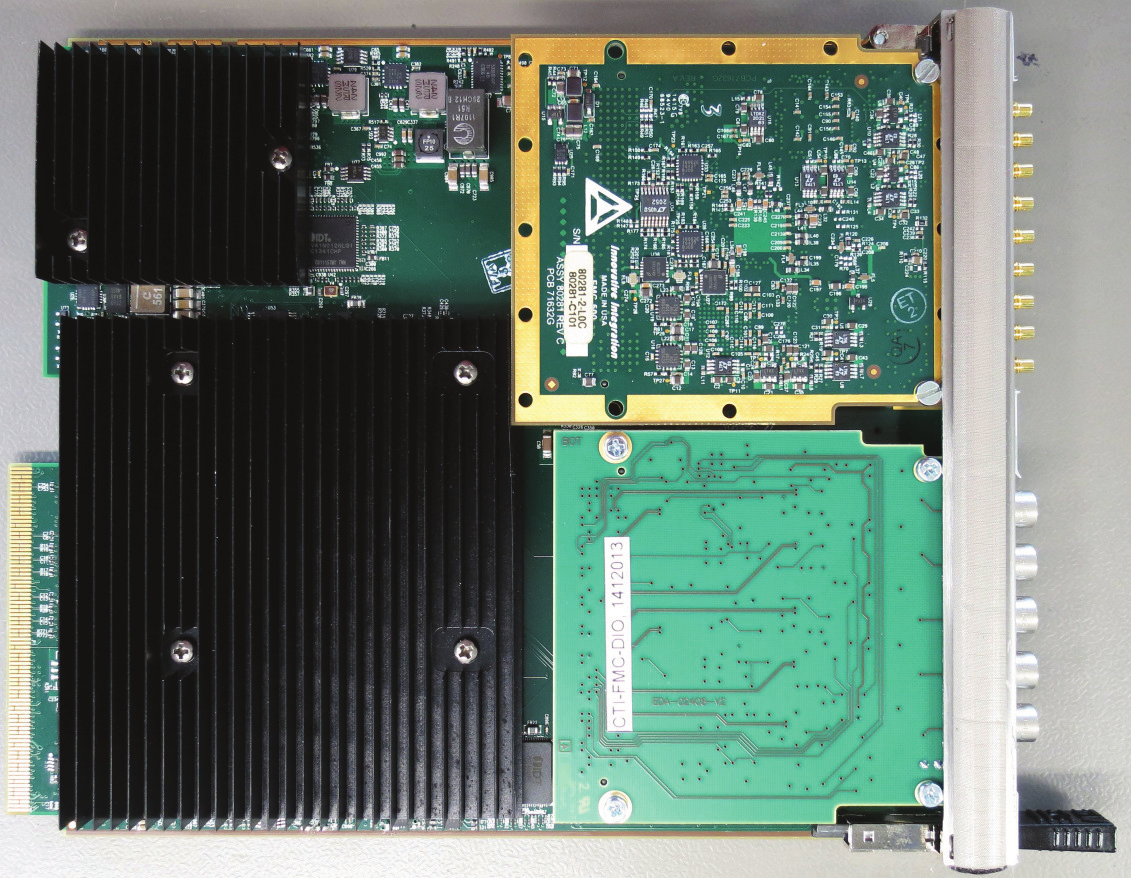
\includegraphics[width=\linewidth]{THPHA115f1.png}
\squarecaption{Photo of assembly of FMC-500 and Digital IO FMC on the AMC525
carrier, with FMC-500 at top right.}
\label{fmc500}
\end{figure}


\begin{figure*} %[!t]
\begin{centering}
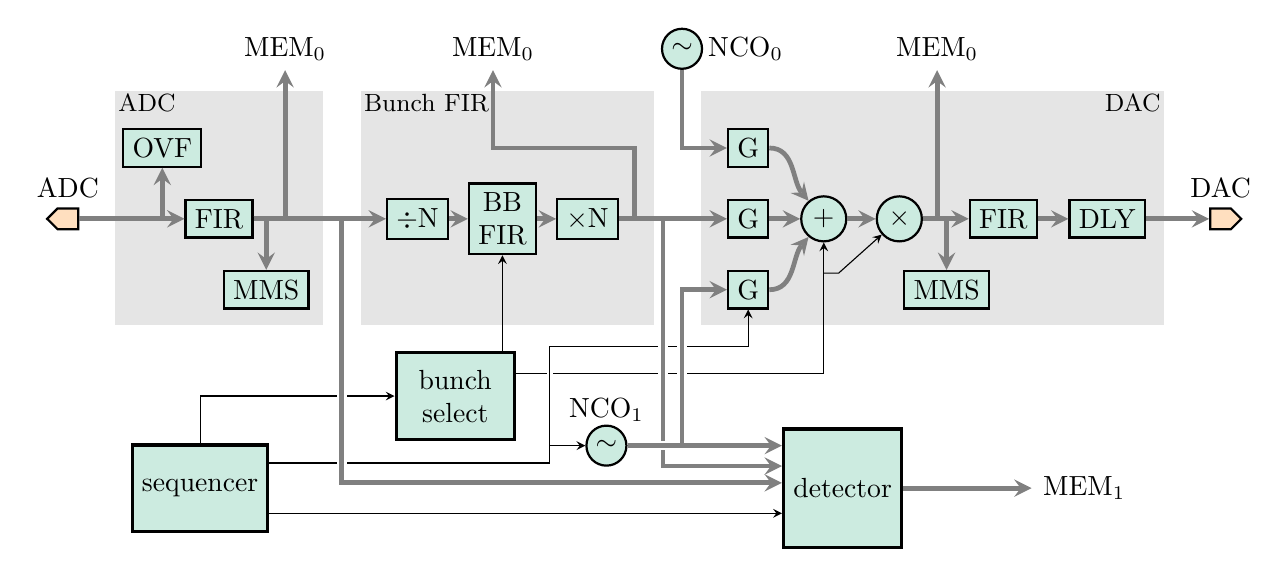
\begin{tikzpicture}[
    transform shape,
    adc-dac/.style={
        draw, single arrow, thick, accent fill,
        single arrow head extend=0pt, shape border rotate=#1},
    area label/.style={anchor=north west, inner sep=1pt, font=\small},
    x=12mm, y=9mm
    ]

    \path [background fill] (0.3,1.8)
        node [area label] {ADC} rectangle ++(2.2,-3.3);
    \path [background fill] (2.9,1.8)
        node [area label] {Bunch FIR} rectangle ++(3.1,-3.3);
    \path [background fill] (6.5,1.8) rectangle ++(4.9,-3.3)
        ++(0,3.3) node [area label, anchor=north east] {DAC};

    \path
        (-0.2,0) node [adc-dac=180, label={ADC}] (adc in) {}
        +(1.0,1) node [small box] (adc ovf) {OVF}
        ++(1.6,0) node [small box] (adc fir) {FIR}
        +(0.5,-1) node [small box] (adc mms) {MMS}
        +(0.7,2.4) node (adc mem) {MEM\textsubscript{0}}
        ++(2.1,0) node [small box] (decimate) {$\div$N}
        ++(0.9,0) node [small box] (bb fir) {BB\\FIR}
        ++(0.9,0) node [small box] (interpolate) {$\times$N}
        +(-1,2.4) node (fir mem) {MEM\textsubscript{0}}
        ++(1.7,0) node [small box] (fir gain) {G}
        +(0,1) node [small box] (nco0 gain) {G}
        +(0,-1) node [small box] (nco1 gain) {G}
        ++(0.8,0) node [mul] (sum) {$+$}
        ++(0.8,0) node [mul] (product) {$\times$}
        +(0.5,-1) node [small box] (dac mms) {MMS}
        +(0.4,2.4) node (dac mem) {MEM\textsubscript{0}}
        ++(1.1,0) node [small box] (dac fir) {FIR}
        ++(1.1,0) node [small box] (delay) {DLY}
        ++(1.2,0) node [adc-dac, label={DAC}] (dac out) {};

    \node [box] at (1.2,-3.8) (sequencer) {sequencer};
    \path (bb fir) ++(-0.5,-2.5) node [box] (bunch) {bunch\\select};
    \node [box, minimum height=15mm] at (8,-3.8) (detector) {detector};
    \path (nco1 gain) ++(-1.5,-2.2)
        node [mul,
            label={[inner sep=1pt]above:NCO\textsubscript{1}}] (nco1) {$\sim$};

    \draw [bus] (adc in) -- (adc fir);
    \draw [bus] (adc in) -| (adc ovf);
    \draw [bus] (adc fir) -| (adc mms);
    \draw [bus] (adc fir) -| (adc mem);
    \draw [bus] (adc fir) -- (decimate);

    \draw [bus] (decimate) -- (bb fir);
    \draw [bus] (bb fir) -- (interpolate);
    \draw [bus] (interpolate) -- (fir gain);
    \draw [bus] (interpolate) ++(0.5,0) -- ++(0,1) -| (fir mem);
    \draw [bus] (fir gain) -- (sum);
    \draw [bus] (nco0 gain) to [out=0, in=130] (sum);
    \draw [bus] (nco1 gain) to [out=0, in=-130] (sum);
    \draw [bus] (sum) -- (product);
    \draw [bus] (product) -- (dac fir);
    \draw [bus] (product) -| (dac mms);
    \draw [bus] (product) -| (dac mem);
    \draw [bus] (dac fir) -- (delay);
    \draw [bus] (delay) -- (dac out);

    \draw [bus, <-] (nco0 gain) -- ++(-0.7,0) -- ++(0,1.4)
        node [mul, label={[inner sep=1pt]right:NCO\textsubscript{0}}] {$\sim$};

    \draw [thin, ->] (sequencer) |- (bunch);
    \draw [thin, ->] (bunch.north-|bb fir) -- (bb fir);
    \draw [thin, <-] (product) -- ++(-130:1) -- (\lastcoord-|sum);
    \draw [thin, ->] (bunch.20) -| (sum);
    \draw [thin, ->] (sequencer.-20) -- (\lastcoord-|detector.west);
    \draw [thin, ->] (sequencer.20) -| ($(nco1)+(-0.6,0)$)
        coordinate (nco1 control) -- (nco1);
    \multipath [thin] {\draw (nco1 control) -- ++(0,1.4);}
    \draw [thin, ->] (nco1 control) -- ++(0,1.4) -| (nco1 gain);

    \multipath [bus] {\draw (interpolate) ++(0.8,0) |- (detector.160);}
    \multipath [bus] {\draw (adc fir) ++(1.3,0) |- (detector.175);}
    \multipath [bus, -] {
        \draw (nco1) -- ++(0.8,0) -- (\lastcoord|-nco1 gain);
        \draw (nco1) -- ++(0.8,0) -- (\lastcoord|-detector.145);
    }
    \draw [bus] (nco1) ++(0.8,0) |- (nco1 gain);
    \draw [bus] (nco1) ++(0.8,0) |- (detector.145);

    \draw [bus] (detector) -- ++(2,0)
        node [anchor=west] {MEM\textsubscript{1}};

\end{tikzpicture}

% vim: filetype=tex:

\end{centering}
\squarecaption{Overview of LMBF signal processing chain.
    Key: \smallbox{OVF}~ADC input overflow detection;
    \smallbox{FIR}~I/O compensation filter;
    \smallbox{MMS}~bunch position and motion measurement;
    \smallbox{$\div$N}~bunch by bunch decimation;
    \smallbox{BB FIR}~bunch by bunch filter;
    \smallbox{$\times$N}~bunch by bunch interpolation;
    \smallbox{G}~gain control;
    \smallbox{DLY}~output alignment delay;
    \smallbox[mul, inner sep=2pt]{$\sim$}~controllable oscillator (NCO).
}
\label{overview}
\end{figure*}



The development of our new LMBF processor was driven by two motivations: to
ensure that we are ready for any new longitudinal instabilities, and to increase
the capabilities of our existing system~\cite{ipac2017rf, ibic2016}.  We also
wanted to improve our knowledge and understanding of high speed processing
hardware relevant to synchrotron diagnostics.

We started with an investigation to determine the appropriate hardware platform
for this kind of development.  Early on it was decided that we would need a
powerful FPGA with FMC (FPGA Mezzanine Card) support.  Initially we looked at
self contained FPGA platforms, and even briefly considered creating our own, but
in the end we converged on MicroTCA~\cite{mtca}.  This platform provides us with
a wide choice of crates and AMC (ATCA Mezzanine Card) processing modules with
high speed interconnect.  The same platform is being used for a joint
development with ALBA of digital low level RF~\cite{ipac2017llrf}.

Having selected MicroTCA as our platform we then selected the following
hardware.  Figure \ref{fmc500} shows the digital processing hardware assembled
ready for insertion in the MicroTCA crate.

\begin{Description}
\item[FMC-500M]
    (HPC) High Pin Count FMC providing dual channel 500\,MS/s 14-bit ADC and
    dual channel 1230\,MS/s 16-bit DAC~\cite{fmc500}.  This will support
    bunch-by-bunch operation at our machine RF frequency of 500\,MHz, and can be
    driven by our machine clock.
\item[FmcDIO5chTTLa]
    Five port digital IO FMC~\cite{fmcdio}.  This is used for miscellaneous
    triggering and other signals.
\item[AMC525]
    Double width AMC card with two HPC FMC slots, 2\,GB of fast on board DRAM
    and 128\,MB of slower DRAM connected to a Virtex-7 690 FPGA, supporting an 8
    lane gen3 PCIe connection over the MicroTCA backplane~\cite{amc525}.  This
    is where all the FPGA firmware will run, and the fast backplane connection
    will allow us to do a lot of data processing in the associated CPU.
\item[AMC720]
    This is an AMC card with an Intel Xeon processor with ample memory and
    sufficient local storage.  We install Red Hat Enterprise Linux 7 on this,
    and run our control system and any associated signal processing.
\item[VT814]
    This is a 2U MicroTCA chassis with 6 AMC slots and dual redundant power
    supplies.
\end{Description}



\section{Functionality and Design}

\subsection{Functionality}

The bunch-by-bunch processor has two functions: to stabilise coupled bunch
oscillations of the electron beam, and to provide diagnostics functions for
measuring beam behaviour and detailed parameters.

Bunch oscillation is stabilised by a feedback filter applied to each bunch to
generate feedback at around 180\textdegree{} out of phase.

For diagnostics our processor provides the following features:
\begin{Itemize}
\item
    Capture of up to 2\,GB of two channels of 500\,MS/s data, selectable from
    different processing stages.  This allows the capture of bunch by bunch
    behaviour and feedback channels.
\item
    Multiple Numerically Controlled Oscillators (NCOs) for driving excitation
    onto the beam.  This is used for tune measurement and grow damp experiments.
\item
    Detectors for capturing IQ data by mixing an NCO with the beam response.
    Outputs from the detectors are written to slow memory and can be used for
    tune measurement and other experiments.
\item
    Programmable sequencer for programming a sequence of NCO frequencies and
    controlling the behaviour of the detectors.
\item
    Individual bunch controls.  For each bunch a different excitation and
    different feedback filter can be selected.  This allows us to perform tune
    measurement on a chosen set of bunches, and to have a different feedback
    filter for a hybrid bunch.
\end{Itemize}

Diagnostics experiments are performed by programming the bunch controls, the
available filters and the sequencer, and then the sequencer is triggered.
Measurements are then written to slow memory and then read out and processed by
the control system.


\subsection{System Design}

Figure \ref{overview} shows the signal processing chain as implemented in the
current design.  This is similar to the existing TMBF as reported
earlier~\cite{icalepcs2015}.  The main enhancements so far (work is still in
progress) are the improved bunch by bunch motion measurement, longer FIR filters
throughout, and rate change to support longitudinal processing.

There are two memory capture targets, MEM\textsubscript0 used for dual channel
full data rate capture, configured as a 2\,GB circular buffer, and
MEM\textsubscript1 used for detector capture, configured as two separate 64\,MB
blocks.

As both the ADC and DAC on the FMC-500 are dual channel, one FPGA image supports
two channels of operation.  In transverse mode of operation the two channels
operate independently on X and Y.


\subsection{Bunch-by-Bunch Min/Max/Sum}

In the earlier design the motion of each bunch is captured by capturing the
minimum and maximum position of each bunch over a 200\,ms interval and
displaying the difference as the beam motion.  In the current design this data
has been extended by accumulating both sum and sum of squares for each bunch
over the sampling interval.

After processing in the control system, this now allows us to display the mean
bunch position and the standard deviation of beam motion.  This provides a more
sensitive view of bunch behaviour.


\subsection{Longitudinal Processing Features}

There is not too much difference in the processing required for longitudinal vs
transverse bunch by bunch feedback --- the biggest differences is in the output
drive chain after the DAC, as described in~\cite{ibic2016}.  However, there are
three signal processing differences that are important to our system.


\subsubsection{Operating on beam phase.}

The input signal to LMBF comes from the sum signal from a set of electron beam
position monitor (EBPM) buttons, processed by a front end to generate two
signals with 90\textdegree{} phase separation, processed as channels $I$ and $Q$
of input.  The front end phase will be controlled to drive the overall signal
level of $Q$ as close to zero as possible.

After this preparation, the signal $I$ should measure the fill pattern, and
$Q$ will measure the phase relative to RF of each bunch (scaled by signal level,
but that's a feature common to all bunch-by-bunch processors).  Longitudinal
feedback is performed on the $Q$ signal alone.


\subsubsection{Generating single side-band IQ.}

In longitudinal mode the output signal will be used to drive a mixer.  To
reduce out of band power demands we will operate with an IQ mixer and will
generate a single side-band feedback signal.

This is done by duplicating the $Q$ input signal onto both processing chains
immediately before bunch-by-bunch FIR processing, and programming the FIRs in
the two channels to generate phase shifts of the synchrotron tune separated by
90\textdegree{}.  The resulting two DAC outputs will drive the IQ mixer.


\subsubsection{Bunch-by-bunch frequency shift.}

The synchrotron tune (longitudinal oscillation frequency) is a low fraction of
the machine revolution frequency, in our case typically around 0.004.  This will
require a substantial frequency shift, which is done by decimation and
interpolation.

Each bunch is averaged for a programmable number of turns before being fed to
the bunch-by-bunch FIR.  The output from the filter is then held stationary for
the same number of turns to generate the up sampled output.


\subsection{Longitudinal vs Transverse Processing}

It is helpful to be able to use the same firmware and software for both
longitudinal and transverse processing.  Switching between these two modes is
done by configuring the decimation and configuring inter-channel operation.

The bunch-by-bunch FIR decimation and interpolation stage is disabled by setting
the decimation count to 1.

There are three inter-channel cross-bars, configured for straight-through
operation in transverse mode, and with the following special settings for
longitudinal operation:
\begin{Itemize}
\item
    The second ADC input channel $Q$ is duplicated onto both processing channels
    immediately before FIR processing.  This allows capture of ADC for $I$, but
    supports operation on the beam phase.
\item
    Only one sequencer is active and is configured to control both channels
    simultaneously.
\item
    The NCO outputs are configured to drive the same signal with 90\textdegree{}
    phase shift into the two outputs, and again only once set of NCOs is active.
\end{Itemize}


\section{Implementation}


\subsection{Interconnect}

\begin{figure}
\begin{centering}
Dataflows through the interconnect

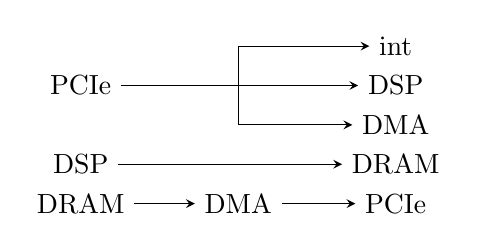
\begin{tikzpicture}[
    baseline,
    x=20mm, y=5mm,
    every path/.style={draw, ->}]

    \path [draw=none]
        (0,0) node (PCIe in) {PCIe}
        +(2,0) node (DSP out) {DSP}
        +(2,1) node (int out) {int}
        +(2,-1) node (DMA out) {DMA}
        ++(0,-2) node (DSP in) {DSP}
        +(2,0) node (DRAM out) {DRAM}
        ++(0,-1) node (DRAM in) {DRAM}
        +(1,0) node (DMA) {DMA}
        +(2,0) node (PCIe out) {PCIe};

    \path (PCIe in) -- (DSP out);
    \path (PCIe in) -- +(1,0) |- (int out);
    \path (PCIe in) -- +(1,0) |- (DMA out);
    \path (DSP in) -- (DRAM out);
    \path (DRAM in) -- (DMA);
    \path (DMA) -- (PCIe out);
\end{tikzpicture}

\medskip
Schematic interconnect implementation
\smallskip

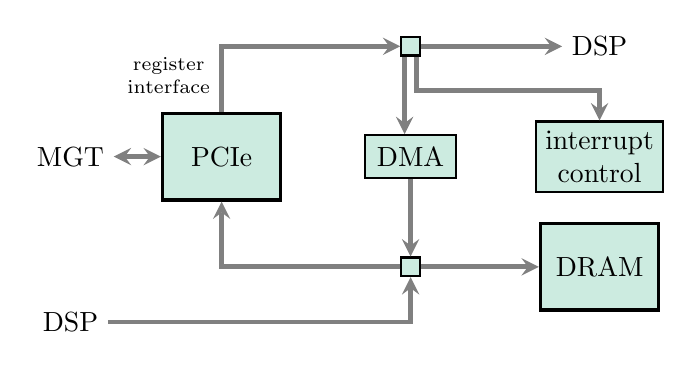
\begin{tikzpicture}[
    x=24mm, y=14mm]

    \path
        (-0.8,0) node (MGT) {MGT}
        (0,0) node [box] (PCIe) {PCIe}
        (1,1) node [small box] (axi lite) {$\varprod$}
        (2,1) node (DSP out) {DSP}
        (1,0) node [small box, inner sep=1ex] (DMA) {DMA}
        (2,0) node [small box] (intr) {interrupt\\control}
        (1,-1) node [small box] (axi) {$\varprod$}
        (2,-1) node [box] (DRAM) {DRAM}
        (-0.8,-1.5) node (DSP in) {DSP};

    \path [bus, <->] (MGT) -- (PCIe);
    \path [bus] (PCIe) |-
        node[below, anchor=north east, font=\scriptsize]
            {register\\interface} (axi lite);
    \path [bus] (axi lite.-120) -- (DMA.north west-|axi lite.-120);
    \path [bus] (axi lite) -- (DSP out);
    \path [bus] (axi lite.-60) |- ($(intr)+(0,0.6)$) -- (intr);
    \path [bus] (DMA) -- (axi);
    \path [bus] (axi) -- (DRAM);
    \path [bus] (axi) -| (PCIe);
    \path [bus] (DSP in) -| (axi);
\end{tikzpicture}

% vim: filetype=tex:

\end{centering}
\squarecaption{Interconnect between PCI Express core (PCIe), memory (DRAM), and
the LMBF data processor (DSP).  \smallbox{$\varprod$}~indicates an AXI crossbar,
arrows point from master to slave.  Data flows are shown at the top of the
figure.}
\label{interconnect}
\end{figure}

After the ``Hello World'' step of getting flashing LEDs, the very first
development was of what we've called the ``Interconnect''.  This part of the
system glues together all of the core resources provided by the FPGA carrier
card to provide a basic environment for the development of the rest of the
system.

Figure \ref{interconnect} illustrates the basic structure of the interconnect.
The register interface is used by the control system to manage the rest of the
processing chain (referred to as DSP here), a simple interrupt controller, and a
DMA engine for transferring data from DRAM to processor memory.

This part of the FPGA design was constructed using the Vivado Block Design
editor, which is a graphical tool for configuring and linking Xilinx components
into a complete design.  The AXI bus is used to connect all of the components.
The rest of the system is written in VHDL.


\subsection{Kernel Driver}

A dedicated kernel driver manages the interface from the processor to this part
of the core FPGA system.  The DSP registers are available to be mapped into
memory, whereas the DMA and interrupt control registers are managed by the
driver only.  This allows for separation between the constantly evolving system
interface, running in user space, and the fixed interrupt and memory management.
Also, it is helpful to separate out the memory and interrupt management, as this
part of the system is able to crash or otherwise compromise the behaviour of the
control processor.

The kernel driver presents three device nodes to userspace, one for mapping
registers into memory and receiving interrupt events, and two for memory readout
from the two banks of DRAM provided by the AMC525.  The design and
implementation of this driver has remained unchanged since the start of the
project.


\subsection{Top Level System Design}

The FPGA design is structured into the interconnect described above
(Fig.~\ref{interconnect}), interfaces to the two FMC cards, two channels of
feedback processing (DSP), and a shared register control interface.  Four banks
of registers provide control over:
\begin{Itemize}
\item
    System level registers for clock management and FMC-500 control and setup.
\item
    Control registers for resources shared between the two DSP channels
    including triggering and fast capture to memory.
\item
    Two banks of registers, one dedicated to each DSP channel.
\end{Itemize}

A custom software tool is used to manage the list of register assignments.  From
a central list of registers and fields, VHDL definitions, C \texttt{struct}
definitions, and documentation are automatically generated.  This makes it
straightforward to add, remove, or rearrange registers, which is otherwise
laborious and error prone.


\subsection{FMC-500 Configuration}

An initial challenge to getting the FMC-500 up and running was that the
documentation for the card~\cite{fmc500} was lacking in important detail; we
understand that the normal application for this component is as part of a vendor
supplied system.  However, the manufacturer was very helpful in answering our
questions and providing the missing pieces.

The FMC-500 is built from three key devices, a PLL clock controller (LMK04828),
a dual channel ADC (AD9684), and a dual channel DAC (AD9122), each of which is
controlled by a dedicated SPI interface.  The ADC and DAC are straightforward to
configure (the DAC is somewhat more complex), but the PLL controller is very
complex.

A Python script captures the complex register interface to the LMK04828 and is
run on the processor during system startup.


\subsection{Signal Processing Chain}

Most of the LMBF signal processing chain was taken from our last TMBF
design~\cite{icalepcs2015}, but nevertheless there has been a lot of rework.
The most important changes to the original design include the following:

\begin{Itemize}
\item
    Beam motion measurement now also measures mean beam position and standard
    deviation of motion.
\item
    Bunch by bunch down and up sampling is now part of the bunch-by-bunch FIR.
    This is needed for LMBF to support the very low synchrotron tune number.
\item
    There are now multiple tune measurement detectors with individual bunch
    enables on each detector.
\item
    Cross-bars are provided at key points in the signal processing chain to
    support IQ processing for LMBF feedback and excitation.
\end{Itemize}


\subsection{Pipelines and Delay Compensation}

For any complex FPGA design it is necessary to pay a lot of attention to
pipelines in the data flow.  Inevitably these introduce delays, and unless
compensated for, there can be data skews between different parts of the system.
In our firmware we have handled these delays and skews by a process of
automated measurement and software compensation.

The skews of interest are those that affect which bunch appears as ``bunch
zero'' in the various readouts and controls, such as the various min/max/sum
waveforms, capture to DRAM, bunch-by-bunch configuration control, and detector
configuration.

We have created a Python script which works through all the relevant
configuration options and automatically measures all the skews.  At the time of
writing the delays cover a range of over 100 RF clock ticks!  The EPICS driver
then uses these measurements to compensate all the waveforms it delivers to
users.


\subsection{EPICS Driver}

The control system runs on the dedicated processor card and provides an EPICS
interface to all aspects of the system.  User interface screens are built using
EDM.


\section{Development Challenges}

\subsection{FPGA Culture Shock}

Coming to FPGA development as a software engineer is a real culture shock.  The
huge differences in semantic model are interesting, but really this is the
smallest issue.  The main challenges are two fold.

Firstly, the state of the art in Hardware Definition Languages (HDLs) is very
weak.  The mainstream languages (VHDL, Verilog, SystemVerilog) all suffer from
very poor abstraction, mismatch between language and target, and excessive
verbosity (VHDL especially).  There does seem to be some work on alternatives,
but unfortunately we come to the second challenge.

All FPGA development is strongly and inextricably tied to vendor tools.  The
general philosophy is that \emph{everything} is licensed.  All components
are referred to as ``IP'' (Intellectual Property), and encryption is widespread.
The whole environment is inimical to open source development and sharing.

In the Accelerator and Large Experimental Physics community we rely on
intellectual sharing for reuse and shared development.  From a management
perspective, sharing is important to help manage the risks associated with the
mismatch between the relatively brief lifetime of modern technology, and the
extended lifetime of large facilities.


\subsection{Development Cycle}

Three challenges stand out in the development cycle: source control, build
times, and debugging.

For source control it is important to separate built from edited files, and it
is desirable to store source files in a format which is friendly to diff.
Although this can be done with the Xilinx Vivado development tool, this process
goes against the grain of the tool.  Scripted development is supported, but the
process is surprisingly fragile.

The build process is extraordinarily slow, particularly in comparison with
compiling a software language.  The process is certainly more complex, and in
particular the placement and routing of resources on the FPGA is difficult.

Debugging FPGA code is more laborious than debugging software, in particular it
is much more difficult to inspect what is going on inside the device, and the
slow build process makes debugging by instrumentation not very practical.
Instead, debugging is mostly done through simulation, and there are some very
sophisticated and complex simulation tools available to complement the
development process.


\subsection{Running at 500\,MHz}

In the previous TMBF design we operated with 4 lanes of digital processing with
an FPGA clock of 125\,MHz.  Implementing this makes for some clumsy
complications in the firmware, so when we discovered that the our new FPGA
supports 500\,MHz operation it was very tempting to simplify the code by
reworking the design for single lane operation.  This might have been unwise.

According to Xilinx documentation, any 7-series FPGA of speed grade 2 supports
500\,MHz operation of the key components, block memory, and DSP units.  However,
there are two main challenges.

The first obstacle was rather unexpected: when allowing Vivado to infer block
memory assignment (the normal way of using this resource), it turns out that the
tool automatically configures the memory in a slower mode of operation which is
not compatible with full speed operation.  This was fixed with an explicit mode
overwrite in the FPGA constraints.

The second obstacle is that achieving timing closure is very hard, and is very
brittle against any changes in the code.  It seems that the component placement
state of the development tool is not well optimised for 500\,MHz placement, and
it needs a lot of manual guidance.  So far this has been done using ``pblocks''
which are used to restrict where certain parts of the design are placed on the
device.


\section{Conclusions}

Development of the new TMBF and LMBF system has been very instructive, and will
provide DLS and other projects with enhanced bunch-by-bunch feedback and
diagnostics capabilities.  We are looking to share this development, and are
actively exploring collaborations with a number of laboratories.

Work is in progess in progress to sort out licensing issues so that we can share
our work freely with other facilities.

We will be extending the diagnostic capabilities of the system described here
with further filtering, with more excitation and detection options, and with
other improvements to be determined.


\begin{thebibliography}{99}

\bibitem{icalepcs2015}
M.G.~Abbott, G.~Rehm, and I.S.~Uzun, \enquote{Architecture of transverse multi-bunch
feedback processor at Diamond}, in \emph{Proc. ICALEPCS'15}, Melbourne, Australia, 
Oct. 2015, pp. 298--301, 
\url{doi: 10.18429/JACoW-ICALEPCS2015-MOPGF097}

\bibitem{dipac2007}
A.F.D.~Morgan, G.~Rehm, and I.~Uzun, \enquote{First tests of the transverse
multibunch feedback at Diamond}, in \emph{Proc. DIPAC'07}, Venice, Italy, May 2017, 
pp. 295--297.

\bibitem{epac2008}
A.F.D.~Morgan, G.~Rehm, and I.~Uzun, \enquote{Performance and features of the
Diamond TMBF system}, in \emph{Proc. EPAC'08}, Genoa, Italy. Jun. 2008, pp. 3281--3283.

\bibitem{biw2010}
G.~Rehm, M.G.~Abbott, A.F.D.~Morgan, J.~Rowland, and I.~Uzun, \enquote{Measurement
of lattice parameters without visible disturbance to user beam at Diamond Light
Source}, in \emph{Proc. BIW'10}, Santa Fe, NM, USA, pp. 44--48.

\bibitem{icalepcs2011}
I.~Uzun, M.G.~Abbott, M.T.~Heron, A.F.D.~Morgan, and G.~Rehm, \enquote{Operational
status of the transverse multibunch feedback system at Diamond}, 
in \emph{Proc. ICALEPCS'11}, Grenoble, France, Oct. 2011, pp. 219--222.

\bibitem{ibic2013}
M.G.~Abbott, G.~Rehm, and I.S.~Uzun, \enquote{Capability upgrade of the Diamond
transverse multibunch feedback}, in \emph{Proc. IBIC'13},
Oxford, UK, Sep. 2013, pp. 682--685.

\bibitem{ibic2014}
G.~Rehm, M.G.~Abbott, and A.F.D~Morgan, \enquote{New features and measurements using
the upgraded transverse multibunch feedback at Diamond}, in \emph{IBIC'14}, 
Monterey, CA, USA, pp. 696--699.

\bibitem{epac2006}
E.~Plouviez, P.~Arnoux, F.~Epaud, J.~Jacob, J.M.~Koch, N.~Michel, G.A.~Naylor,
J.\mbox{-}L.~Revol, V.~Serriere, and D.~Vial, \enquote{Broadband bunch by bunch
feedback for the ESRF using a single high resolution and fast sampling FPGA
DSP}, in \emph{Proc. EPAC'06}, Edinburgh, UK, Jun. 2006, pp. 2976--2978.

\bibitem{libera}
Instrumentation Technologies, \enquote{Libera Bunch-by-Bunch},
\url{http://www.i-tech.si}

\bibitem{ipac2017rf}
C.~Christou \emph{et al.}, \enquote{Progress with the Diamond Light Source RF upgrade},
in \emph{Proc. IPAC'17},  Copenhagen, Denmark, May 2017, pp. 4358--4361,\\
\url{doi: 10.18429/JACoW-IPAC2017-THPIK112}

\bibitem{ibic2016}
G.~Rehm, M.G.~Abbott, and A.F.D.~Morgan, \enquote{Measurements of longitudinal
coupled bunch instabilities and status of new feedback system}, 
in \emph{Proc. IBIC'16}, Barcelona, Spain, Sep. 2016, pp. 298--301, \\
\url{doi: 10.18429/JACoW-IBIC2016-TUCL03}

\bibitem{mtca}
MicroTCA Overview, PICMG, \\
\url{https://www.picmg.org/openstandards/microtca/}.

\bibitem{ipac2017llrf}
P.~Gu \emph{et al.}, \enquote{Digital low level RF systems for Diamond Light Source},
in \emph{Proc. IPAC'17}, Copenhagen, Denmark, May 2017, pp. 4089--4091,\\
\url{doi: 10.18429/JACoW-IPAC2017-THPAB152}


\bibitem{fmc500}
Innovative Integration, \enquote{FMC-500, FMC Module with 2x 500 MSPS 14-bit
A/D, 2x 1230 MSPS 16-bit DACs with PLL and Timing Controls},
\url{https://www.innovative-dsp.com/products.php?product=FMC-500}

\bibitem{fmcdio}
CERN Open Hardware Repository, \enquote{FMC DIO 5ch TTL a},
\url{https://www.ohwr.org/projects/fmc-dio-5chttla}

\bibitem{amc525}
Vadatech, \enquote{AMC525, dual FMC carrier, 2 FMC, 690T FPGA, FFG-1761 package,
FPGA Mezzanine Card}, \\
\url{http://vadatech.com/product.php?product=393}


\end{thebibliography}


\end{document}
